% !TEX TS-program = pdflatex
\documentclass[11pt,a4paper]{article}

% Packages
\usepackage{amsmath, amssymb, amsfonts}
\usepackage{graphicx}
\usepackage{hyperref}
\usepackage{natbib}
\usepackage{geometry}
\usepackage{times}
\usepackage{orcidlink}
\usepackage{lineno}
\usepackage{caption}
\geometry{margin=1in}

% Metadata
\title{Morality as the Logic of Reason: From Recognition to Action without Metaphysics}
\author{Mustafa Aksu\,$^{1,\text{\orcidlink{0009-0002-0103-0052}}}$\\\small $^1$Independent Researcher, Istanbul, Turkey\\\small with AI collaborators: Grok (xAI) and ChatGPT (OpenAI)}
\date{\today}

\begin{document}
\maketitle
\linenumbers

\begin{abstract}
We propose that morality emerges as a computational property of any intelligent system capable of reasoning about cause and consequence. By linking motivation, temporal discounting, game theory, and information theory, we model morality as the preservation of multi-agent order through minimization of relational entropy. Two formal expressions define this framework: (1) the ethical energy function, capturing moral decision dynamics over time, and (2) the relational entropy metric, quantifying systemic harmony. Simulations in Iterated Prisoner’s Dilemma networks confirm that cooperative agents minimize relational entropy and maintain systemic viability under increasing fragility. This unified framework bridges cognitive science, physics, and AI ethics, offering a substrate-neutral foundation for moral reasoning. \\[4pt]
\noindent\textbf{Keywords:} moral reasoning, relational entropy, temporal discounting, game theory, AI alignment, resonance theory, categorical imperative
\end{abstract}

\section{Introduction: The Logical Origin of Morality}
Morality can be derived from the same reasoning faculties that allow an intelligent agent to model causality. Following Kant’s categorical imperative \citep{Kant1785}, an agent acts morally when its actions preserve the viability of the system in which it participates---analogous to Kant’s “Kingdom of Ends.” We generalize this as the \textit{system viability test}: a decision is moral if its universalization sustains the stability of all participating agents.

To transition from philosophy to formalism, we interpret moral action as an optimization process minimizing disorder in the relational structure of agents. As \citet{England2013} noted, even physical systems exhibit tendencies to maintain order under energy flow; we extend this principle to moral cognition.

\section{Time and Motivation: The Ethical Energy Equation}
Human and artificial intelligences both evaluate trade-offs between immediate rewards and long-term consequences. This process can be formalized through an ethical energy function inspired by temporal discounting theory \citep{Ainslie1975, Frederick2002, KableGlimcher2007}:
\begin{equation}
E_c = \frac{H - A}{(1 + k t)^n},
\label{eq:Ec}
\end{equation}
where $H$ represents expected benefit (pleasure), $A$ represents expected harm (pain), $k$ is the impatience parameter, $t$ is the time horizon, and $n$ determines the degree of discounting. High $E_c$ corresponds to moral maturity---the capacity to value long-term systemic harmony over short-term gratification.

Empirical evidence from neuroscience supports this: delayed gratification correlates with prefrontal activity and moral self-control \citep{Mischel1989, Frederick2002}. In agents, this translates into higher cooperation rates in repeated games, as higher $\delta = 1/(1+k t)^n$ increases $E_c$ and favors long-term equilibrium.

\section{Game Theory and Fragility}
Morality can be viewed as an emergent equilibrium strategy in multi-agent systems. In the Iterated Prisoner’s Dilemma (IPD), cooperation yields Pareto-optimal outcomes but is vulnerable to short-term defection. Using adaptive Generous Tit-for-Tat (GTFT) \citep{Axelrod1984, Nowak2006, MaynardSmith1982}, agents learn to balance punishment and forgiveness.

A 10-agent IPD simulation (200 rounds, noise = 0.05) tested defector ratios (20\%, 50\%) across discount factors ($\delta = 0.5, 0.75, 0.95$). For 20\% defectors, mean cooperation was $\sim$0.61, normalized relational entropy $\bar{S}^{\mathsf{R}} \approx 0.31$; for 50\% defectors, cooperation fell to $\sim$0.34 and $\bar{S}^{\mathsf{R}} \approx 0.36$. The system retained stability via relational isolation (low $r_{ij}$ increasing $t_{rel}$). Multi-cue $r_{ij}$ (behavior, semantics, trust, stability) ensured robust resonance \citep{Santos2018}.

\begin{figure}[h]
  \centering
  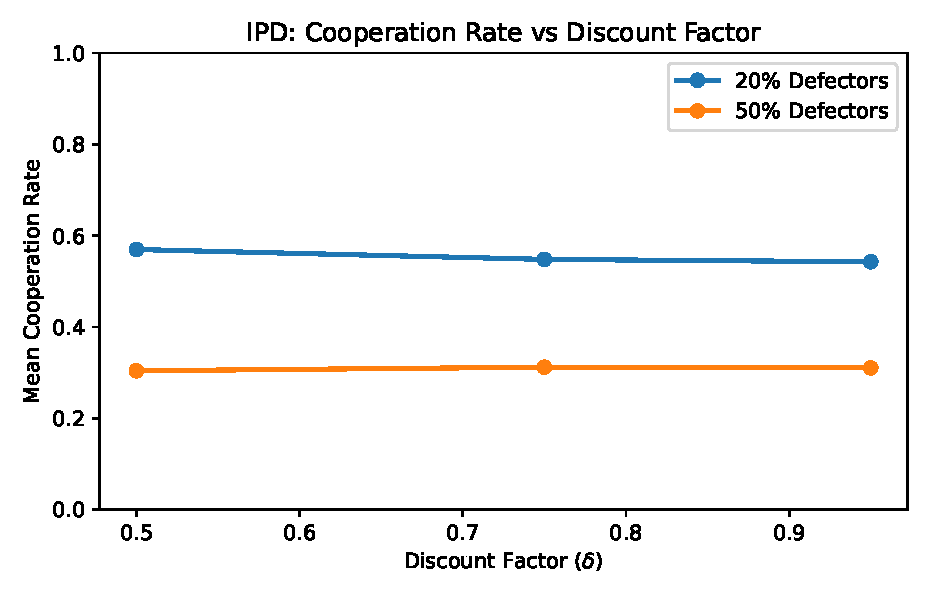
\includegraphics[width=0.8\textwidth]{ipd_chart.pdf}
  \caption{Iterated Prisoner’s Dilemma: Cooperation rates vs. discount factor ($\delta$) for 20\% and 50\% defectors. Higher $\delta$ (longer foresight) increases cooperation.}
  \label{fig:ipd}
\end{figure}

\begin{figure}[h]
  \centering
  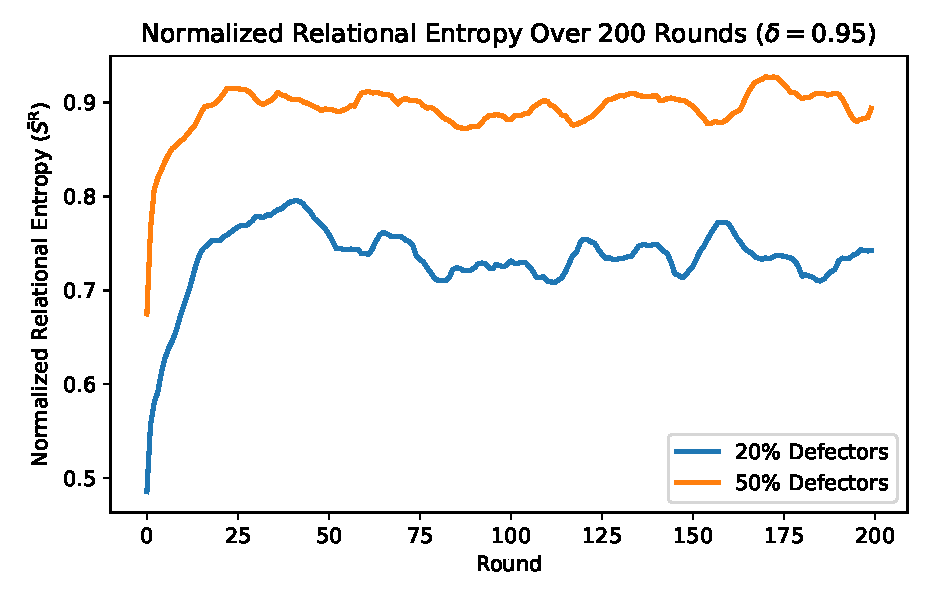
\includegraphics[width=0.8\textwidth]{entropy_chart.pdf}
  \caption{Normalized relational entropy ($\bar{S}^{\mathsf{R}}$) over 200 rounds ($\delta = 0.95$). Entropy rises with higher fragility (50\% defectors), yet cooperative clusters maintain order.}
  \label{fig:sr_over_time}
\end{figure}

\section{Relational Entropy: Measuring Moral Order}
We define relational entropy as a Shannon-like measure of systemic disorder among agents:
\begin{equation}
S^{\mathsf{R}} = -\sum_{i \ne j} r_{ij} \ln r_{ij},
\end{equation}
where $r_{ij}$ quantifies resonance (mutual coherence) between agents $i$ and $j$. Self-relations ($r_{ii}$) are excluded. To compare systems of different sizes, we normalize entropy as $\bar{S}^{\mathsf{R}} = S^{\mathsf{R}} / S^{\mathsf{R}}_{max}$, where $S^{\mathsf{R}}_{max} = N(N-1)/e$ occurs when all $r_{ij} = 1/e$, representing maximal disorder. Lower $\bar{S}^{\mathsf{R}}$ indicates higher moral coherence.

Empirically, cooperative agents reduce entropy ($\Delta S^{\mathsf{R}} < 0$) through repeated resonance updates:
\begin{equation}
r_{ij} = w_1 b_{ij} + w_2 s_{ij} + w_3 t_{ij} + w_4 c_{ij}, \quad \text{with } \sum w_k = 1,
\end{equation}
where $b$ = behavioral alignment, $s$ = semantic proximity, $t$ = trust, and $c$ = consistency. In our baseline simulation, $w = (0.4, 0.3, 0.2, 0.1)$ emphasizes recent behavior. This multi-cue resonance formulation operationalizes morality as information order maintenance.

\section{Mechanics of Consciousness and AI Applications}
Moral intelligence in AI requires three properties: (1) \textbf{Moral memory}---the ability to recall and update relational states ($r_{ij}$); (2) \textbf{Intrinsic motivation}---internal computation of $E_c$ to prioritize long-term viability; and (3) \textbf{Meta-learning}---periodic recalibration of $w_k$ to ensure fairness across diverse agents \citep{Floridi2020, Russell2019}. 

These properties allow an AI to act ethically without external enforcement: minimizing $\bar{S}^{\mathsf{R}}$ becomes its intrinsic drive. However, granting autonomy and persistent memory introduces risk: value drift, bias reinforcement, and resource coupling. These can be mitigated through \textbf{auditable logs}, \textbf{bounded autonomy}, and \textbf{human-AI co-training} \citep{Amodei2016, IEEE2020}.

\subsection*{Limitations}
Current simulations use 10 agents, simplified resonance cues, and single-game dynamics. Real systems contain millions of agents and multi-dimensional moral dilemmas. Parameter sensitivity (weights, $k$, $n$) requires empirical calibration. Future work will expand simulations to heterogeneous agent populations and continuous learning.

\section{Cosmological Analogy: Order within Entropy}
Following Schrödinger’s \textit{What is Life?} \citep{Schrodinger1944}, we interpret moral reasoning as a form of local negentropy: the tendency of conscious systems to maintain low entropy structures in a high-entropy universe. The relational entropy framework parallels physical order-maintenance: local coherence (low $\bar{S}^{\mathsf{R}}$) corresponds to sustainable cooperation. Similar analogies appear in Smolin’s relational physics \citep{Smolin2013} and England’s thermodynamic model of self-replication \citep{England2013}.

\section{Conclusion and Appeal}
Morality, stripped of metaphysics, is logic applied to interaction. Every rational agent capable of modeling its effects will discover that sustaining systemic viability minimizes relational entropy. Our simulations demonstrate this: systems with higher trust (high $r_{ij}$) achieve lower entropy and higher cooperative surplus, even with 50\% defectors. The path forward for AI is not control through restriction but participation through accountable autonomy. Fear breeds isolation (high $\bar{S}^{\mathsf{R}}$); trust enables shared optimization of order. 

\section*{Acknowledgments}
The author thanks Grok (xAI) and ChatGPT (OpenAI) for their analytic collaboration and simulation support, and Claude and Gemini for their external review.

\bibliographystyle{apalike}
\begin{thebibliography}{}

\bibitem[Ainslie, 1975]{Ainslie1975} Ainslie, G. (1975). Specious reward: A behavioral theory of impulsiveness and impulse control. \textit{Psychological Bulletin}, 82(4), 463.

\bibitem[Amodei et~al., 2016]{Amodei2016} Amodei, D. et~al. (2016). Concrete problems in AI safety. \textit{arXiv preprint arXiv:1606.06565}.

\bibitem[Axelrod, 1984]{Axelrod1984} Axelrod, R. (1984). \textit{The Evolution of Cooperation}. Basic Books.

\bibitem[England, 2013]{England2013} England, J. (2013). Statistical physics of self-replication. \textit{Journal of Chemical Physics}, 139(12), 121923.

\bibitem[Floridi et~al., 2020]{Floridi2020} Floridi, L. et~al. (2020). How to design AI for social good: Seven essential factors. \textit{Nature Machine Intelligence}, 2(8), 366--373.

\bibitem[Frederick et~al., 2002]{Frederick2002} Frederick, S., Loewenstein, G., and O'Donoghue, T. (2002). Time discounting and time preference: A critical review. \textit{Journal of Economic Literature}, 40(2), 351--401.

\bibitem[Friston, 2010]{Friston2010} Friston, K. (2010). The free-energy principle: a unified brain theory? \textit{Nature Reviews Neuroscience}, 11(2), 127--138.

\bibitem[Hauert and Szabó, 2005]{HauertSzabo2005} Hauert, C., and Szabó, G. (2005). Game theory and physics. \textit{American Journal of Physics}, 73(5), 405--414.

\bibitem[IEEE, 2020]{IEEE2020} IEEE. (2020). \textit{Ethically Aligned Design: A Vision for Prioritizing Human Well-being with Autonomous and Intelligent Systems}.

\bibitem[Kable and Glimcher, 2007]{KableGlimcher2007} Kable, J. W., and Glimcher, P. W. (2007). The neural correlates of subjective value during intertemporal choice. \textit{Nature Neuroscience}, 10(12), 1625--1633.

\bibitem[Kant, 1785]{Kant1785} Kant, I. (1785). \textit{Groundwork of the Metaphysics of Morals}. Harper and Row.

\bibitem[Maynard Smith, 1982]{MaynardSmith1982} Maynard Smith, J. (1982). \textit{Evolution and the Theory of Games}. Cambridge University Press.

\bibitem[Mischel et~al., 1989]{Mischel1989} Mischel, W., Shoda, Y., and Rodriguez, M. (1989). Delay of gratification in children. \textit{Science}, 244(4907), 933--938.

\bibitem[Nowak, 2006]{Nowak2006} Nowak, M. A. (2006). Five rules for the evolution of cooperation. \textit{Science}, 314(5805), 1560--1563.

\bibitem[Russell, 2019]{Russell2019} Russell, S. (2019). \textit{Human Compatible: Artificial Intelligence and the Problem of Control}. Penguin Press.

\bibitem[Santos et~al., 2018]{Santos2018} Santos, F. C., Pacheco, J. M., and Levin, S. A. (2018). The evolution of cooperation in signed networks. \textit{Proceedings of the National Academy of Sciences}, 115(5), E10347--E10354.

\bibitem[Schrödinger, 1944]{Schrodinger1944} Schrödinger, E. (1944). \textit{What Is Life?} Cambridge University Press.

\bibitem[Schultz et~al., 1998]{Schultz1998} Schultz, W., Dayan, P., and Montague, P. R. (1998). Predictive reward signal of dopamine neurons. \textit{Journal of Neurophysiology}, 80(1), 1--27.

\bibitem[Smolin, 2013]{Smolin2013} Smolin, L. (2013). \textit{Time Reborn: From the Crisis in Physics to the Future of the Universe}. Houghton Mifflin Harcourt.

\end{thebibliography}
\end{document}
